\renewcommand*{\arraystretch}{1.1}

\subsection*{BI / read / 21}
\label{section:bi-read-21}

\renewcommand{\currentQueryCard}{21}
    \marginpar{
	\raggedleft
	\vspace{0.22ex}

    \queryRefCard{bi-read-01}{BI}{1}\\
    \queryRefCard{bi-read-02}{BI}{2}\\
    \queryRefCard{bi-read-03}{BI}{3}\\
    \queryRefCard{bi-read-04}{BI}{4}\\
    \queryRefCard{bi-read-05}{BI}{5}\\
    \queryRefCard{bi-read-06}{BI}{6}\\
    \queryRefCard{bi-read-07}{BI}{7}\\
    \queryRefCard{bi-read-08}{BI}{8}\\
    \queryRefCard{bi-read-09}{BI}{9}\\
    \queryRefCard{bi-read-10}{BI}{10}\\
    \queryRefCard{bi-read-11}{BI}{11}\\
    \queryRefCard{bi-read-12}{BI}{12}\\
    \queryRefCard{bi-read-13}{BI}{13}\\
    \queryRefCard{bi-read-14}{BI}{14}\\
    \queryRefCard{bi-read-15}{BI}{15}\\
    \queryRefCard{bi-read-16}{BI}{16}\\
    \queryRefCard{bi-read-17}{BI}{17}\\
    \queryRefCard{bi-read-18}{BI}{18}\\
    \queryRefCard{bi-read-19}{BI}{19}\\
    \queryRefCard{bi-read-20}{BI}{20}\\
    \queryRefCard{bi-read-21}{BI}{21}\\
    \queryRefCard{bi-read-22}{BI}{22}\\
    \queryRefCard{bi-read-23}{BI}{23}\\
    \queryRefCard{bi-read-24}{BI}{24}\\
    \queryRefCard{bi-read-25}{BI}{25}\\
}



\noindent\begin{tabularx}{\queryCardWidth}{|>{\queryPropertyCell}p{\queryPropertyCellWidth}|X|}
	\hline
	query & BI / read / 21 \\ \hline
%
	title & Zombies in a country
 \\ \hline
%
	pattern & \hfill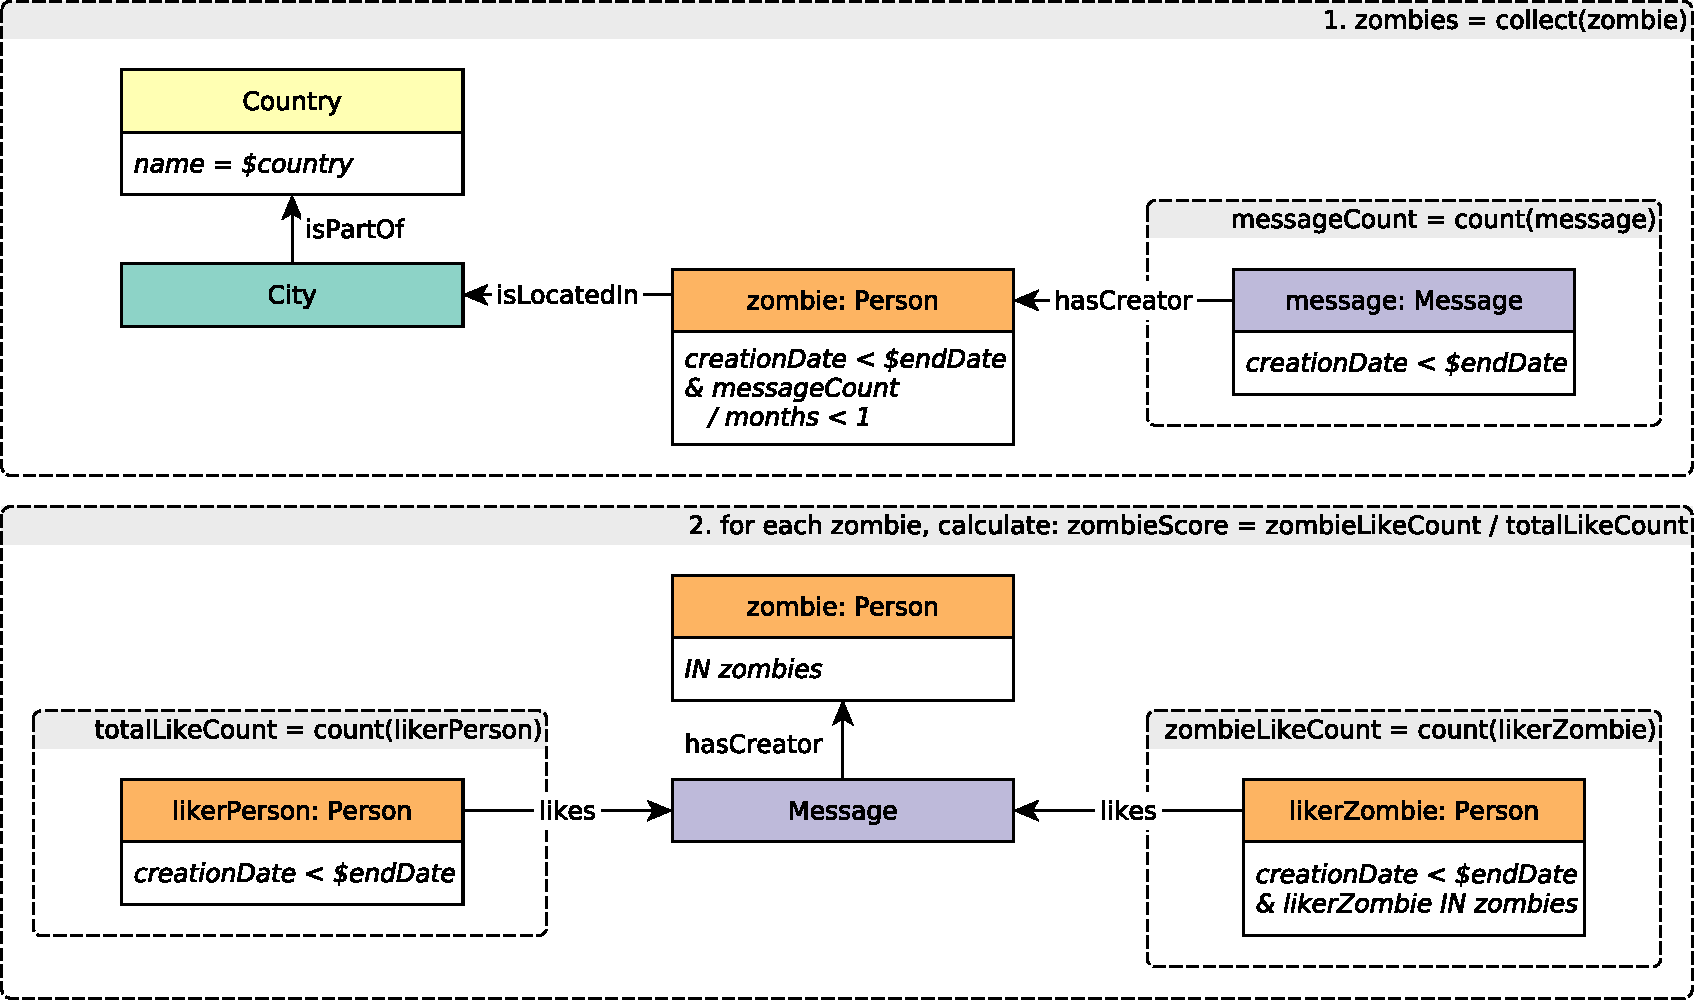
\includegraphics[scale=\patternscale,margin=0cm .2cm]{patterns/bi-read-21}\hfill\vadjust{} \\ \hline
%
	desc. & Find zombies within the given \texttt{country}, and return their zombie
scores.

A \texttt{zombie} is a \emph{Person} created before the given
\texttt{endDate}, which has created an average of \texttt{{[}0,\ 1)}
\emph{Messages} per month, during the time range between profile
creation date and the given \texttt{endDate}. The number of months spans
the time range from creation date of the profile to the \texttt{endDate}
with partial months on both end counting as one month (e.g.~a
\texttt{creationDate\ of} Jan 31 and an \texttt{endDate} of Mar 1
results in 3 months).

For each \texttt{zombie}, calculate the following:

\begin{itemize}
\tightlist
\item
  \texttt{zombieLikeCount}: the number of likes received from other
  zombies
\item
  \texttt{totalLikeCount}: the total number of likes received on that
  \texttt{zombie}'s \emph{Messages}
\item
  \texttt{zombieScore}: \texttt{zombieLikeCount} /
  \texttt{totalLikeCount}
\end{itemize}

For both \texttt{zombieLikeCount} and \texttt{totalLikeCount}, only
count likes received from profiles that were created before the given
\texttt{endDate}.
 \\ \hline
%
	
		params &
		\innerCardVSpace{\begin{tabularx}{\attributeCardWidth}{|>{\paramNumberCell}c|>{\varNameCell}M|>{\typeCell}m{\typeWidth}|Y|} \hline
		$\mathsf{1}$ & country
 & String
 &  \\ \hline
		$\mathsf{2}$ & endDate
 & Date
 &  \\ \hline
		\end{tabularx}}\innerCardVSpace \\ \hline
	
%
	
		result &
		\innerCardVSpace{\begin{tabularx}{\attributeCardWidth}{|>{\resultNumberCell}c|>{\varNameCell}M|>{\typeCell}m{\typeWidth}|>{\resultOriginCell}c|Y|} \hline
		$\mathsf{1}$ & zombie.id & 64-bit Integer & R &
				 \\ \hline
		$\mathsf{2}$ & zombieLikeCount & 32-bit Integer & A &
				 \\ \hline
		$\mathsf{3}$ & totalLikeCount & 32-bit Integer & A &
				 \\ \hline
		$\mathsf{4}$ & zombieScore & 32-bit Float & A &
				The ratio of \texttt{zombieLikeCount} and \texttt{totalLikeCount}
 \\ \hline
		\end{tabularx}}\innerCardVSpace \\ \hline
	
%
	
		sort		&
		\innerCardVSpace{\begin{tabularx}{\attributeCardWidth}{|>{\sortNumberCell}c|>{\varNameCell}M|>{\directionCell}c|Y|} \hline
		$\mathsf{1}$ & zombieScore
 & $\desc
$ &  \\ \hline
		$\mathsf{2}$ & zombie.id
 & $\asc
$ &  \\ \hline
		\end{tabularx}}\innerCardVSpace \\ \hline
	%
	limit & 100 \\ \hline
	%
	CPs &
	\multicolumn{1}{>{\raggedright}l|}{
		\chokePoint{1.2}, 
		\chokePoint{2.1}, 
		\chokePoint{2.3}, 
		\chokePoint{2.4}, 
		\chokePoint{3.2}, 
		\chokePoint{3.3}, 
		\chokePoint{5.1}, 
		\chokePoint{5.3}
		} \\ \hline
	%
	%
\end{tabularx}
\queryCardVSpace